%------------------------------------------------------
%Author             : Daniel Schembri, Jonathan Schwarz
%University         : Pforzheim University
%Date of last edit  : Wed, 03 Sep 2014 14:12:16 +0200
%Filename           : multithreading_with_posix_pthreads.tex
%------------------------------------------------------

\documentclass[10pt,a4paper,DIV=11]{scrreprt}

%British English
\usepackage[UKenglish]{babel}
%utf8
\usepackage[utf8]{inputenc}

%Multicolumn lists
\usepackage{multicol}

%pseudo-code
\usepackage[boxruled,vlined]{algorithm2e}

%for source code listings
\usepackage{listings}

\usepackage[table]{xcolor}

%tikz
\usepackage{tikz}
\usetikzlibrary{arrows,positioning,fit}

%plots
\usepackage{pgfplots}

%blocks - used by tikz-uml, included before
\pgfdeclarelayer{background}
\pgfdeclarelayer{foreground}
\pgfsetlayers{background,main,foreground}

%<,> in tikz-uml
\usepackage[T1]{fontenc}
\usepackage{tikz-uml}

%subfigure
\usepackage{graphicx}
\usepackage{subfigure}

%prevent figure from floating pictures
\usepackage{float}

%footer & header
\usepackage{fancyhdr}

%push footer down
\usepackage[bottom]{footmisc}

%footer & header
\pagestyle{fancy}
%clean footer & header
\fancyhf{}

%bibtex
\usepackage[square,numbers]{natbib}
\usepackage{gensymb}

%equation
\usepackage[tbtags]{amsmath}
\usepackage{amssymb} 

%table of contents with hyperlinks
%always include as last package
\usepackage{hyperref}

%===========================TITLE PAGE=======================================

%university logo
\titlehead
{

%    Pforzheim University\\
 %   School of Engineering\\
}

%\subject{Project work}
	
\title
{
    Instructions to use the simulator\\
}

\author
{
    by \textbf{Daniel Schembri} - matriculation number: 310026
}
\date
{
    Summer term 2015 \\
  %  \today{}
}


\publishers
{
    Examiner: Prof. Dr. Richard Alznauer\\
    Supervisor: Dr. Christoph Ussfeller
}


%=========================================GLOBAL SETTINGS=========================================

%footer &header

%\fancyfoot[L]{\textbf{Multi-Threading mit POSIX-pThreads}}
\fancyhead[R]{Page \thepage}
%\fancyhead[L]{\thechapter}

%chapter number and title
\fancyhead[L]{\nouppercase{\leftmark}}
%line
%\renewcommand{\footrulewidth}{0.5 pt}
\usepackage{lmodern}
\addtokomafont{sectioning}{\rmfamily}
\setlength{\parindent}{0mm}

%colour definitions
\definecolor{dkgreen}{rgb}{0,0.6,0}
\definecolor{gray}{rgb}{0.7,0.7,0.7}
%medium gray
\definecolor{mgray}{gray}{0.80}
%light gray
\definecolor{lgray}{gray}{0.97}

%hyperlink settings
%frame around hyperlinks
\hypersetup
{
    colorlinks = false,
    linkcolor = black,
    hypertexnames = false,
    citecolor = green
}

%listing settings
\lstset
{ 
    language=C++,                
    basicstyle=\footnotesize\ttfamily,           
    numbers=left,
    stepnumber=5,    
    firstnumber=1,
    numberfirstline=true                 
    numberstyle=\color{black},                 
    numbersep=5pt,                 
    backgroundcolor=\color{white},      
    showspaces=false,             
    showstringspaces=false,         
    showtabs=false,                
    frame=single,                   
    rulecolor=\color{black},       
    tabsize=2,                     
    captionpos=b,                   
    breaklines=true,                
    breakatwhitespace=false,       
    title=\lstname,                    
    keywordstyle=\color{blue},          
    commentstyle=\color{dkgreen}, 
    identifierstyle=\color{black},      
    stringstyle=\color{purple},      
    escapeinside={\%*}{*)},      
    morekeywords={*,...},            
    deletekeywords={...}             
}

\setcounter{tocdepth}{4}  %a deeper contentsmenue
%=====================================DOCUMENT START=========================
\begin{document}

\tikzstyle{line}=[draw]
\tikzstyle{arrow}=[draw, -latex] 

\maketitle
\thispagestyle{empty}
\newpage
{\large\tableofcontents}
\newpage

\chapter{Compilation of the simulator}
\begin{Large}
The compilation was tested under Linux Ubuntu (64-bit): \\


\fbox{
	\begin{minipage}{15cm}
		\begin{enumerate} 
			\item \textbf{Get all necessary packages} \\
			sudo apt-get install git \\(optional for downloading the simulator from github) \\
			sudo apt-get install cmake \\
			sudo apt-get install build-essential \\
			sudo apt-get install xorg-dev \\
			sudo apt-get install freeglut3-dev
			\item \textbf{Unzip the simulator or clone from github} \\
			git clone  \href{http://github.com/Jonathan-Schwarz/neural_networks}{http://github.com/Jonathan-Schwarz/neural\_networks}
			\item \textbf{Go to neural\_networks/new\_graphic/}
			\item \textbf{make}
			\item \textbf{./new\_graphic}
		\end{enumerate}
	\end{minipage}
}   \\
\\ \\
For compilation on other Linux systems equivalent packages as listed in Nr. 1 one have to be installed.


\end{Large}
\normalsize

\chapter{Using the simulator}
\begin{LARGE}
In this chapter the functions of the simulator are described.

As follows a figure of the simulation in progress: \\

\begin{center}
	\begin{figure}[H]
		\centering
		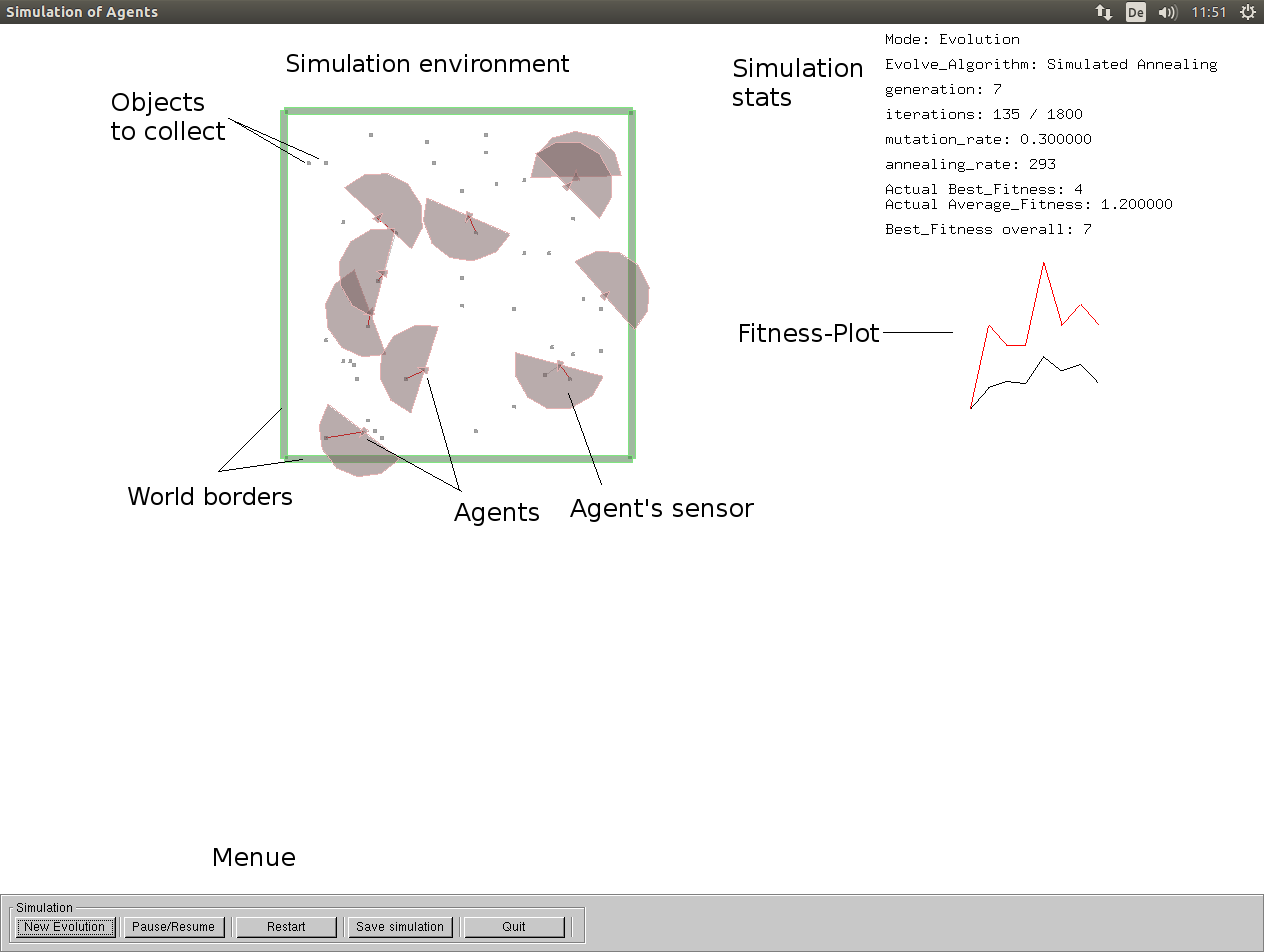
\includegraphics[width=1.0\textwidth,scale=1]{simuinaction.png}  
		\caption{The simulator}
		\label{fig:simulator}
	\end{figure}
\end{center}

The simulator has three parts: the menue, the simulation environment and the stats.
\section{The menue}
On the bottom side there is the menue. As follows the description of the buttons: \\
\textbf{New evolution} \\ Opens a window to choose parameters and start the simulation: \\

\begin{center}
	\begin{figure}[H]
		\centering
		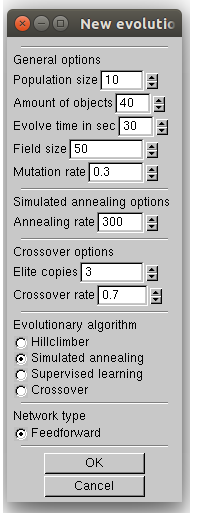
\includegraphics[width=0.28\textwidth,scale=1]{New_Evolution_menu.png}  
		\caption{Create a new simulation}
		\label{fig:evolution}
	\end{figure}
\end{center}

The 'new evolution'-window lets you choose the simulation parameters and the desired algorithm.
After pressing 'OK' the simulation will begin instantly

\textbf{Pause/Resume} \\ Pausing/Resuming the simulation

\textbf{Restart} \\Restarts the complete simulation process with the choosen parameters

\textbf{Save simulation} \\Saves the actual state of the simulation; including parameters, stats and the weights and fitness of each agent in the 'simulation.txt'-file in the programs folder

\textbf{Quit} \\
Quit the program

\newpage

\section{Interacting with the simulation environment}
The simulation environment is displayed in the middle of the window.
To interact with the simulator some specified keys and the mouse can be used. To use them the focus has to be on the simulation environment. Therefore it has to be clicked on the simulation area. As follows the mouse- and key-interactions are described: \\

\textbf{Holding left mouse-button} \\
Click with the left mouse-button on an object or agent, hold it and move the cursor to move it:

\begin{center}
	\begin{figure}[H]
		\centering
		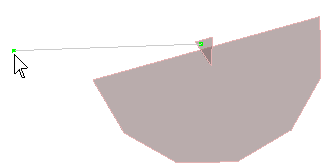
\includegraphics[width=0.6\textwidth,scale=1]{sim_leftmouse.png}  
		\caption{Moving an agent}
		\label{fig:leftmouse}
	\end{figure}
\end{center}



\textbf{Holding right mouse-button} \\
Scrolling through the world 

\textbf{'x'- and 'y'-key} \\
Zooming in/out

\textbf{'p'-key} \\
Pausing/Resuming the simulation 

\textbf{'t'-key} \\
Turbo-mode is enabled/disabled.
In turbo-mode only the stats are updated. The display of the simulation will be frozen as long as the turbo-mode is enabled 

\textbf{'ESC'} \\
Quit the program

\section{The stats}
On the right side there are shown the simulation stats and the fitness plot.
The stats contain information like the choosen algorithm, algorithm specific parameters, the amount of processed generations, fitness values, etc.
The fitness plot is automatically resized with increasing generations to fit in the plotting area. The red plot shows the best fitness for each generation. The grey one shows the average fitnesses.


\end{LARGE}


\end{document}
